\documentclass[lettersize,journal]{IEEEtran}

\usepackage{amsmath,amssymb,amsfonts}
\usepackage{algorithm}
\usepackage[noend]{algpseudocode}
\usepackage{array}
\usepackage{siunitx}
\usepackage{booktabs}
\usepackage{multirow}
\usepackage{makecell}
\usepackage[caption=false,font=normalsize,labelfont=sf,textfont=sf]{subfig}
\usepackage{textcomp}
\usepackage{stfloats}
\usepackage{url}
\usepackage{graphicx}
\usepackage{balance}
\usepackage[T1]{fontenc} % 保证英文字体加粗有效

% 新增的包
\usepackage[table]{xcolor}
\usepackage{placeins}
\hyphenation{op-tical net-works semi-conduc-tor IEEE-Xplore}
\def\BibTeX{{\rm B\kern-.05em{\sc i\kern-.025em b}\kern-.08em
    T\kern-.1667em\lower.7ex\hbox{E}\kern-.125emX}}

\begin{document}

\title{TMSKD: Temporal--Memory Structure-Aware Knowledge Distillation for Liquid Neural Network-based Underwater Acoustic Target Recognition}

\author{Author Name(s) Omitted for Review}

\markboth{IEEE Journal of Oceanic Engineering}%
{TMSKD for Liquid Neural Network-based Underwater Acoustic Target Recognition}

\maketitle

\begin{abstract}
\bfseries
Deep learning has substantially advanced underwater acoustic target recognition (UATR), yet deploying complex deep models on resource-constrained underwater platforms remains challenging. Knowledge distillation (KD) alleviates this issue by transferring knowledge from a high-performance teacher model to a lightweight student model. However, existing KD methods for UATR often neglect the intrinsic multi-scale temporal structure of acoustic signals, limiting temporal modeling capability and recognition performance. To address this problem, this paper proposes a Temporal--Memory Structure-Aware Knowledge Distillation (TMSKD) framework based on Liquid Neural Networks (LNNs). The framework adopts an LNN as the student model to provide strong neural dynamic modeling capability and integrates two complementary distillation strategies: Temporal Separation with Learnable Temperature Knowledge Distillation (TS-T), which enhances time-step-wise semantic distribution alignment, and Memory-Discrepancy Knowledge Distillation (MemKD), which enforces memory-aware alignment to preserve robust discriminative information across time scales. Extensive experiments on two real-world ocean acoustic data sets demonstrate that TMSKD outperforms existing KD methods, achieving 92.39\% accuracy (ACC) on ShipsEar, which improves over the competitive baseline result of 90.03\% by 2.36 percentage points. Notably, TMSKD significantly improves the recognition accuracy of the LNN student model by 9.67 percentage points.
\end{abstract}

\begin{IEEEkeywords}
\bfseries
Underwater acoustic target recognition, knowledge distillation, liquid neural networks, temporal modeling, model compression.
\end{IEEEkeywords}

\section{Introduction}
\IEEEPARstart{U}{nderwater} Acoustic Target Recognition (UATR) is a core technology for marine monitoring and defense systems, and plays an important role in ocean resource exploration, underwater security, and ecological environment monitoring~\cite{Urick1983,Jensen2011}. Compared with terrestrial acoustic environments, underwater acoustic channels are affected by time-varying propagation, multipath effects, and severe environmental noise~\cite{Wenz1962,Medwin2005}. These factors make underwater acoustic signals highly non-stationary and nonlinear, greatly increasing the difficulty of extracting robust and discriminative features from raw signals~\cite{Urick1983,Jensen2011}. More importantly, practical UATR systems are often deployed on edge platforms such as autonomous underwater vehicles, buoys, and sensor nodes, where storage capacity and computational energy consumption are strictly constrained~\cite{Cai2020MobileAUV,Han2016DeepCompression}. Therefore, designing lightweight recognition models under limited computational resources is a critical problem in this field.
\begin{figure}
    \centering
    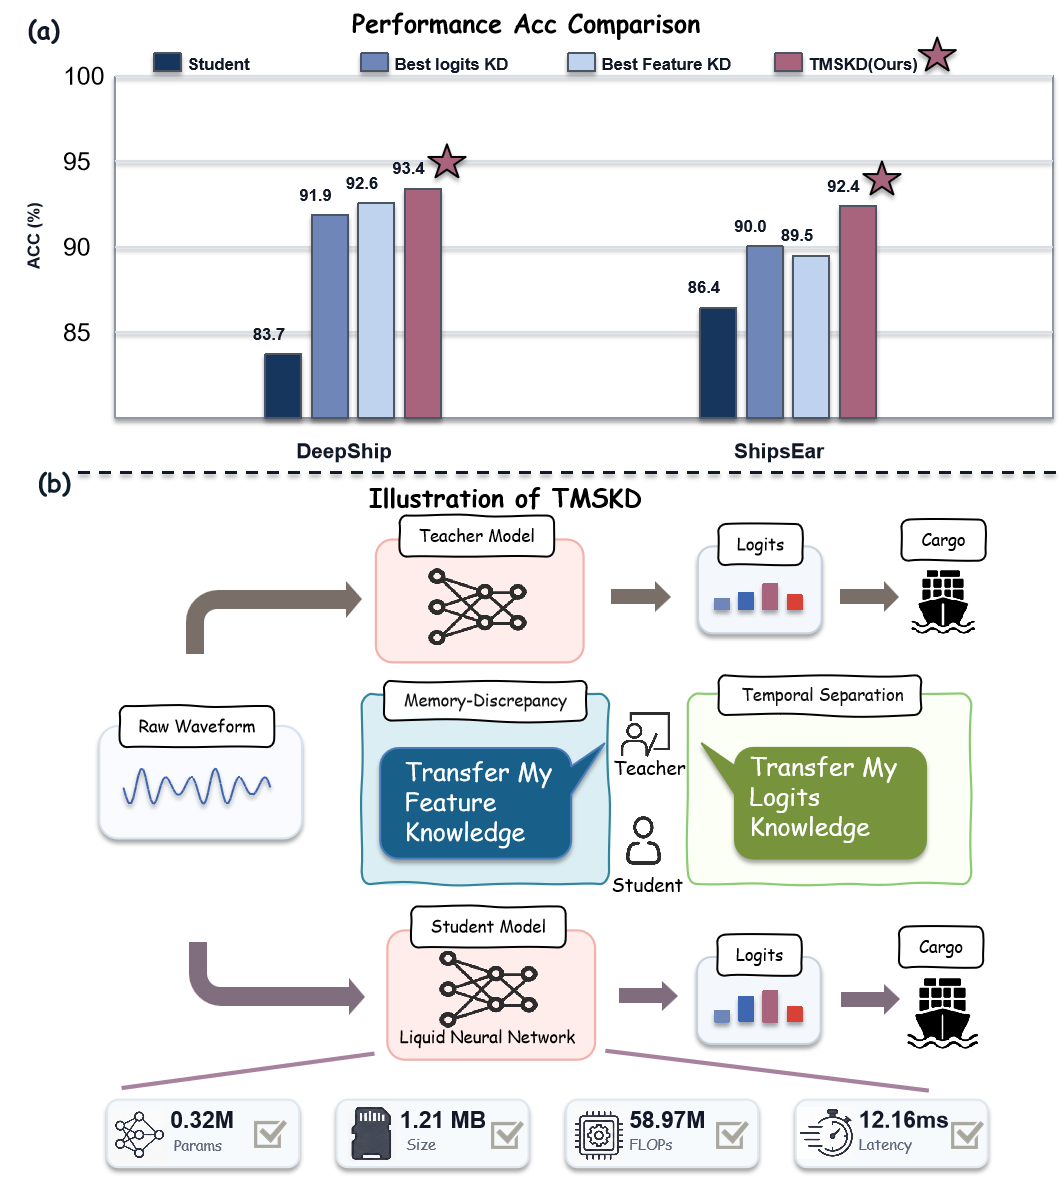
\includegraphics[width=1\linewidth]{figures/Cover_Image.png}
    \caption{
    (a) Accuracy comparison of the original student model, the best-performing logit-based KD method, the best-performing feature-based KD method, and TMSKD on the DeepShip and ShipsEar datasets. TMSKD achieves the highest recognition accuracy on both datasets. (b) Conceptual illustration of TMSKD. The teacher transfers temporal logit knowledge through temporal separation and feature-level dynamic knowledge through memory-discrepancy modeling, jointly guiding the liquid neural network-based student. The resulting student maintains a compact architecture with only 0.32M parameters, a model size of 1.21 MB, 58.97M FLOPs, and an inference latency of 12.16 ms.
    }
    \label{fig:placeholder}
\end{figure}
To address the dual challenges of data scarcity and lightweight deployment, existing studies mainly adopt pretrained model fine-tuning or model compression techniques~\cite{Kong2020PANNs,Gou2021KDSurvey}. Unlike speech or general acoustic signals, however, underwater acoustic signals lack explicit semantic information and phoneme structures. Directly transferring lightweight pretrained models from the general audio domain therefore often fails to capture the physical characteristics of underwater signals, resulting in limited fine-tuning performance~\cite{Baevski2020Wav2Vec2,Kong2020PANNs,Urick1983,Jensen2011,Medwin2005}. Knowledge distillation has consequently become a promising direction, in which a teacher network guides a lightweight student network to improve performance without increasing inference cost~\cite{Bucila2006Compression,Hinton2015Distilling,Romero2015FitNets}. Although prior studies have made progress in applying KD to underwater acoustics, most lightweight student networks still rely on two-dimensional time-frequency features, such as Mel-spectrograms, as input. This strategy exploits visual texture patterns in spectrograms, but introduces costly preprocessing and weakens the end-to-end lightweight design objective. In contrast, lightweight models that directly process one-dimensional raw waveforms often have weaker feature extraction capability than spectrogram-based methods, making it difficult to obtain competitive recognition accuracy under distillation~\cite{Oord2016WaveNet,Bai2018TCN}.

This raises a natural question: can an architecture directly process raw underwater acoustic waveforms while maintaining feature extraction capability comparable to spectrogram-based methods? We answer this question by introducing Liquid Neural Networks (LNNs) into the UATR student model. LNNs are biologically inspired continuous-time recurrent neural networks that model neural dynamics with ordinary differential equations (ODEs)~\cite{Chen2018NeuralODE,Hasani2021LTC,Hasani2022CfC}. Their temporal causality modeling and robustness make them suitable for non-stationary one-dimensional underwater acoustic signals.

To fully exploit the potential of LNNs in UATR and address knowledge transfer between heterogeneous teacher and student architectures, this paper proposes a Memory-Discrepancy Knowledge Distillation (MemKD) module. In conventional feature distillation, direct feature-map alignment can be difficult because teacher and student networks may differ substantially in parameter scale and architecture~\cite{Yim2017FSP,Zagoruyko2017AT,Ahn2019VID}. Such hard alignment may lead to unstable convergence or suboptimal features. MemKD instead transfers the temporal evolution trend of teacher features in an explicit manner. In other words, the student learns not only the teacher's final prediction, but also the dynamic pattern by which the teacher processes acoustic features over time, thereby alleviating the alignment difficulty caused by architectural heterogeneity.

In addition, underwater acoustic signals contain transient characteristics, where specific key frequencies or short-time events may directly determine the target category. These discriminative cues are unevenly distributed along the temporal axis and are easily weakened by conventional logit-based distillation, which usually aligns only the final output distributions. To address this issue, we introduce Temporal Separation with Adaptive Temperature Knowledge Distillation (TS-T), which constrains the semantic distribution consistency between teacher and student along the time dimension. Specifically, the teacher logits are broadcast to each student time step and aligned with the student time-step logits, enabling the student to capture when critical acoustic changes occur. Moreover, TS-T adopts Z-score-normalized logits, where the logit standard deviation serves as a parameter-free adaptive temperature to dynamically adjust distribution smoothness~\cite{Sun2024LSKD}. A learnable fusion coefficient further balances the time-step sequential distillation loss and the final-logit distillation loss, allowing the student to learn both fine-grained temporal cues and stable final decision knowledge.

The main contributions of this paper are summarized as follows:
\begin{enumerate}
    \item We propose a novel KD framework, termed Temporal--Memory Structure-Aware Knowledge Distillation (TMSKD), specifically designed for UATR. TMSKD integrates logits-based Temporal Separation with Adaptive Temperature Knowledge Distillation (TS-T) and feature-based Memory-Discrepancy Knowledge Distillation (MemKD), enabling the student to capture both instantaneous inter-class relationships and long-term temporal memory patterns in underwater acoustic signals.
    \item We design a lightweight and efficient student architecture based on LNNs. The student consists of a five-layer CNN encoder, a Bidirectional Parallel Cross-Slice CfC (BPCSCfC) module with neural circuits automatically generated by AutoNCP, and a Dual-Resolution Attentive Statistics Pooling (DRASP) module. DRASP jointly models global stationary information and local transient cues, improving discriminative sequence representation.
    \item Extensive experiments on two real-world ocean acoustic data sets, ShipsEar and DeepShip, show that the proposed TMSKD significantly outperforms state-of-the-art KD methods while maintaining very low computational complexity and parameter overhead. The results validate its effectiveness and practicality for resource-constrained underwater deployment.
\end{enumerate}

\section{Related Work}
\subsection{Underwater Acoustic Target Recognition}
UATR aims to automatically classify and recognize vessels, underwater vehicles, and other targets by analyzing underwater acoustic signals. It is a key technology for underwater monitoring and marine security~\cite{David2016ShipsEar,Irfan2021DeepShip}. Because underwater propagation environments are complex, the signals often exhibit strong non-stationarity, long-term dependence, and background noise interference, making the task highly challenging~\cite{Urick1983,Jensen2011,Medwin2005}.

Early methods mainly relied on handcrafted time-domain, frequency-domain, and time-frequency features combined with conventional classifiers~\cite{David2016ShipsEar,Chen2021LOFAR}. Although effective in controlled scenarios, such methods strongly depend on manual experience and have limited generalization ability.

Convolutional, recurrent, and Transformer-based deep networks have been widely applied to underwater acoustic recognition, learning discriminative features from time-frequency representations or self-supervised embeddings~\cite{Chen2021LOFAR,TFTokenViT,MHTUATR}. Nevertheless, these models usually use discrete-time modeling and therefore have difficulty capturing continuous-time dynamic characteristics. Meanwhile, transfer learning based on pretrained speech and general-audio models~\cite{Baevski2020Wav2Vec2,Kong2020PANNs} has also been introduced to underwater acoustics to exploit general acoustic representation capability~\cite{ALSIUATR,CAFJTUATR}. Despite these advances, existing methods still face model redundancy, insufficient dynamic modeling, and deployment inefficiency in complex marine environments. Constructing parameter-efficient models with continuous-time dynamic modeling capability is therefore an important research direction.

\subsection{Liquid Neural Networks}
Liquid Neural Networks are continuous-time neural computation models inspired by the dynamics of small biological nervous systems~\cite{Hasani2021LTC}. Their core idea is to describe the state evolution of neurons over time through linear or nonlinear ODEs, thereby modeling temporal signals in a more natural way~\cite{Chen2018NeuralODE}. Unlike conventional networks built from stacked discrete layers, LNNs update hidden states continuously at each time step, which gives them stronger dynamic adaptability and interpretability. Closed-form continuous-time formulations further reduce the cost of numerical ODE solvers while preserving expressive power~\cite{Hasani2022CfC}. Moreover, structured sparse connection strategies, such as automatic neural circuit generation, allow LNNs to achieve efficient dynamic modeling with a small number of parameters~\cite{Lechner2020NCP}.

LNNs have shown strong performance in time-series prediction, robot control, and low-power embedded systems~\cite{Lechner2020NCP,Hasani2021LTC,Hasani2022CfC}. However, their use in UATR remains limited. Introducing LNNs into underwater acoustic recognition can enhance the model's dynamic response to non-stationary signals while satisfying lightweight deployment requirements.

\subsection{Knowledge Distillation}
Knowledge distillation is an effective model compression and performance transfer technique based on a teacher--student framework~\cite{Bucila2006Compression,Hinton2015Distilling,Gou2021KDSurvey}. It uses soft labels or intermediate representations learned by a stronger teacher model to guide the training of a smaller student model, allowing the student to achieve higher recognition accuracy while maintaining low computational complexity. Classical KD aligns softened output distributions using Kullback--Leibler (KL) divergence and a temperature coefficient. Later studies extended KD to feature, attention, and relational distillation, improving generalization by constraining intermediate features or sample relations~\cite{Romero2015FitNets,Zagoruyko2017AT,Park2019RKD}.

For temporal tasks, distillation based only on final-output alignment cannot fully exploit dynamic information along the time dimension. Time-aware distillation strategies have therefore been developed to align predictions or hidden states at each time step~\cite{Farhadi2019TKD,Wang2023TSKD}. Temperature adjustment and soft-label reweighting can further reduce optimization difficulty caused by teacher--student distribution mismatch~\cite{Sun2024LSKD,Zhou2021WSLD}. In UATR, where the input signal contains strong temporal dependence and dynamic variation, combining KD with temporal modeling is beneficial for transferring the discriminative ability of large pretrained models to lightweight dynamic networks.

\section{Methodology}
This section first introduces the LNN-based underwater acoustic recognition structure, and then describes the proposed TMSKD framework, which combines TS-T and MemKD.

\begin{figure*}[!t]
    \centering
    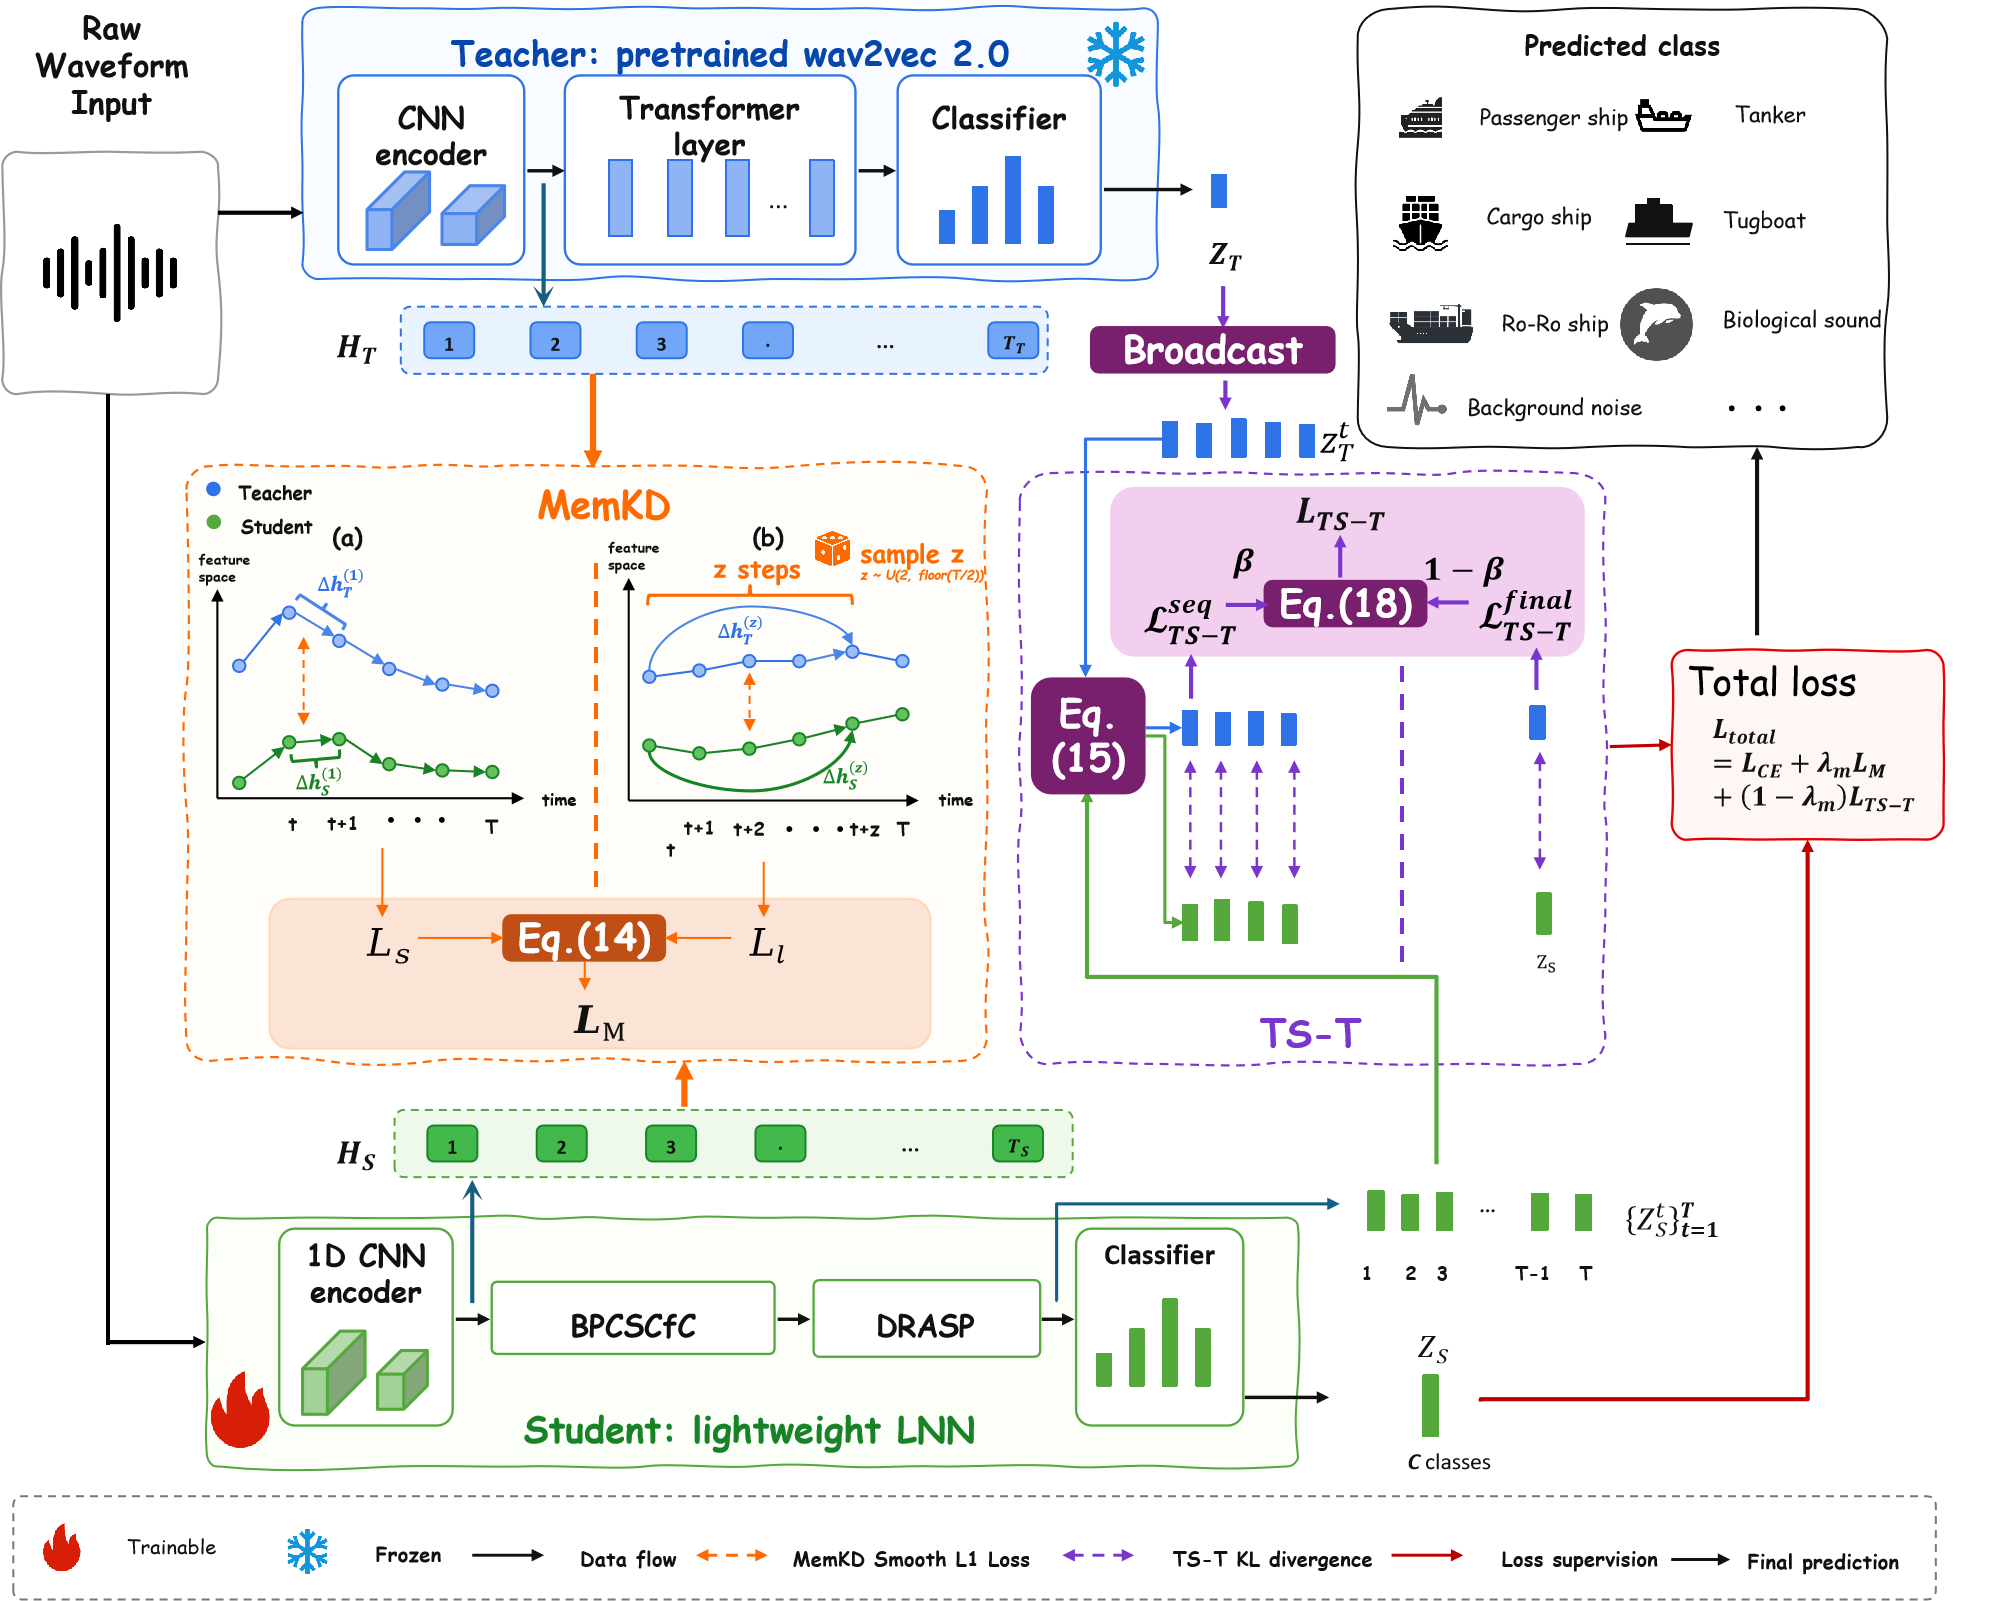
\includegraphics[width=0.92\textwidth]{figures/model_structure_v2.0.png}
    \caption{The overall architecture of the proposed knowledge distillation framework. A frozen pretrained wav2vec 2.0 acts as the teacher model to guide the training of the lightweight LNN student network via Memory-Discrepancy Knowledge Distillation (MemKD) and Temporal Separation with Adaptive Temperature Knowledge Distillation (TS-T). The detailed internal structure of the student network is shown in Fig.~\ref{fig:student_architecture}.}
    \label{fig:structure}
\end{figure*}

\subsection{Preliminaries: Liquid Neural Dynamics}
Underwater acoustic signals are strongly non-stationary and contain complex temporal structures with both local transients and long-range dependencies. Our method adopts a closed-form continuous-time neural network framework~\cite{Hasani2022CfC}. At time $\mathbf{t}$, the neural dynamics describe the temporal evolution of neuron state $\mathbf{x}(t)$ using the following linear first-order differential equation:
\begin{equation}
\frac{d x(t)}{dt} =
-\left[ \tau + f(x(t), I(t), t, \theta) \right] \cdot x(t)
+ f(x(t), I(t), t, \theta) \cdot A,
\label{eq:lnn_ode}
\end{equation}
where $\tau \in \mathbb{R}^C$ is a time constant controlling the changing rate and sensitivity of neural signals, $\theta$ denotes learnable parameters, $I(t)$ is the external input, $f(x(t), I(t), t, \theta)$ is a nonlinear activation function, and $A$ is a learnable vector that scales the nonlinear response. This equation describes the dynamic evolution of neurons under continuous-time decay and external driving, improving expressiveness and adaptability for temporal tasks.

Direct numerical integration of (\ref{eq:lnn_ode}) is computationally expensive. Therefore, a closed-form solution can convert the continuous-time dynamic system into an explicit update in discrete time steps, achieving efficient and stable sequence modeling while retaining continuous-time advantages. Specifically, the approximate analytical solution at time step $t$ is
% \begin{equation}
% \mathbf{x}(t) =
% \sigma\left(-f(\mathbf{x}, \mathbf{I}; \theta_f) t\right) \odot g(\mathbf{x}, \mathbf{I}; \theta_g)
% + \left[1 - \sigma\left(-\left[f(\mathbf{x}, \mathbf{I}; \theta_f)\right] t\right)\right] \odot h(\mathbf{x}, \mathbf{I}; \theta_h),
% \label{eq:cfc_update}
% \end{equation}
\begin{equation}
\begin{split}
\mathbf{x}(t) =& \sigma\left(-f(\mathbf{x}, \mathbf{I}; \theta_f) t\right) \odot g(\mathbf{x}, \mathbf{I}; \theta_g) \\
& + \left[1 - \sigma\left(-\left[f(\mathbf{x}, \mathbf{I}; \theta_f)\right] t\right)\right] \odot h(\mathbf{x}, \mathbf{I}; \theta_h),
\end{split}
\label{eq:cfc_update}
\end{equation}
where $\sigma(\cdot)$ is the sigmoid gating function, $\odot$ denotes element-wise multiplication, $g(x, I; \theta_g)$ extracts instantaneous nonlinear features from the current input $I$ and previous state $x$, and $h(x, I; \theta_h)$ provides a complementary feature representation. Compared with ODE-solver-based networks, this closed-form design is at least one order of magnitude faster. Relative to RNNs or Transformers with fixed discrete time steps, it explicitly models continuous-time dynamics and can flexibly adjust the temporal modeling scale according to input variations, which is particularly suitable for multi-scale and non-stationary underwater acoustic signals.

\paragraph{Neural Circuit Policy}
In UATR, input signals often contain redundant background components and non-stationary noise. To improve robustness and parameter efficiency, liquid neurons are not fully connected. Instead, Auto Neural Circuit Policy (AutoNCP) is used to construct a structured sparse topology~\cite{Lechner2020NCP}. AutoNCP adopts a hierarchical architecture with sensory neurons, interneurons, command neurons, and motor neurons. Sensory neurons correspond to the input feature dimension, while inter, command, and motor neurons form three learnable internal processing layers through sparse random connections. Recurrent connections in the command neuron layer enhance the dependence on historical hidden states. The liquid neuron cells based on (\ref{eq:cfc_update}) evolve on the connection graph defined by AutoNCP, reducing parameter scale while preserving dynamic modeling capability.

\subsection{Student Network for Underwater Acoustic Recognition}
\label{subsec:student}
For a single-channel raw underwater acoustic signal $\mathbf{s} \in \mathbb{R}^{L}$, the student network first uses a one-dimensional CNN encoder to map the raw waveform into high-dimensional temporal features $\mathbf{H}_S \in \mathbb{R}^{B \times T_S \times C}$, where $B$ is the batch size, $T_S$ is the number of time steps, and $C$ is the feature dimension~\cite{Oord2016WaveNet,Bai2018TCN}. To jointly capture fine-grained local transients and long-range temporal dependencies in $\mathbf{H}_S$, we feed it into the BPCSCfC module. The BPCSCfC module divides the sequence along the temporal dimension into non-overlapping windows and constructs parallel information streams to capture both short-range and long-range temporal dependencies. As illustrated in Fig.~\ref{fig:student_architecture}, the resulting multi-scale temporal representation is aggregated by DRASP through complementary global and segment-wise attentive statistics pooling before classification. The complete forward procedure of the student network is summarized in Algorithm~\ref{alg:student_network}. The encoder feature $\mathbf{H}_S$ is used by MemKD, while the fused feature $\mathbf{F}_S^t$ is linearly projected into the time-step logits $\mathbf{Z}_S^t$ used by TS-T.

\begin{figure*}[!t]
    \centering
    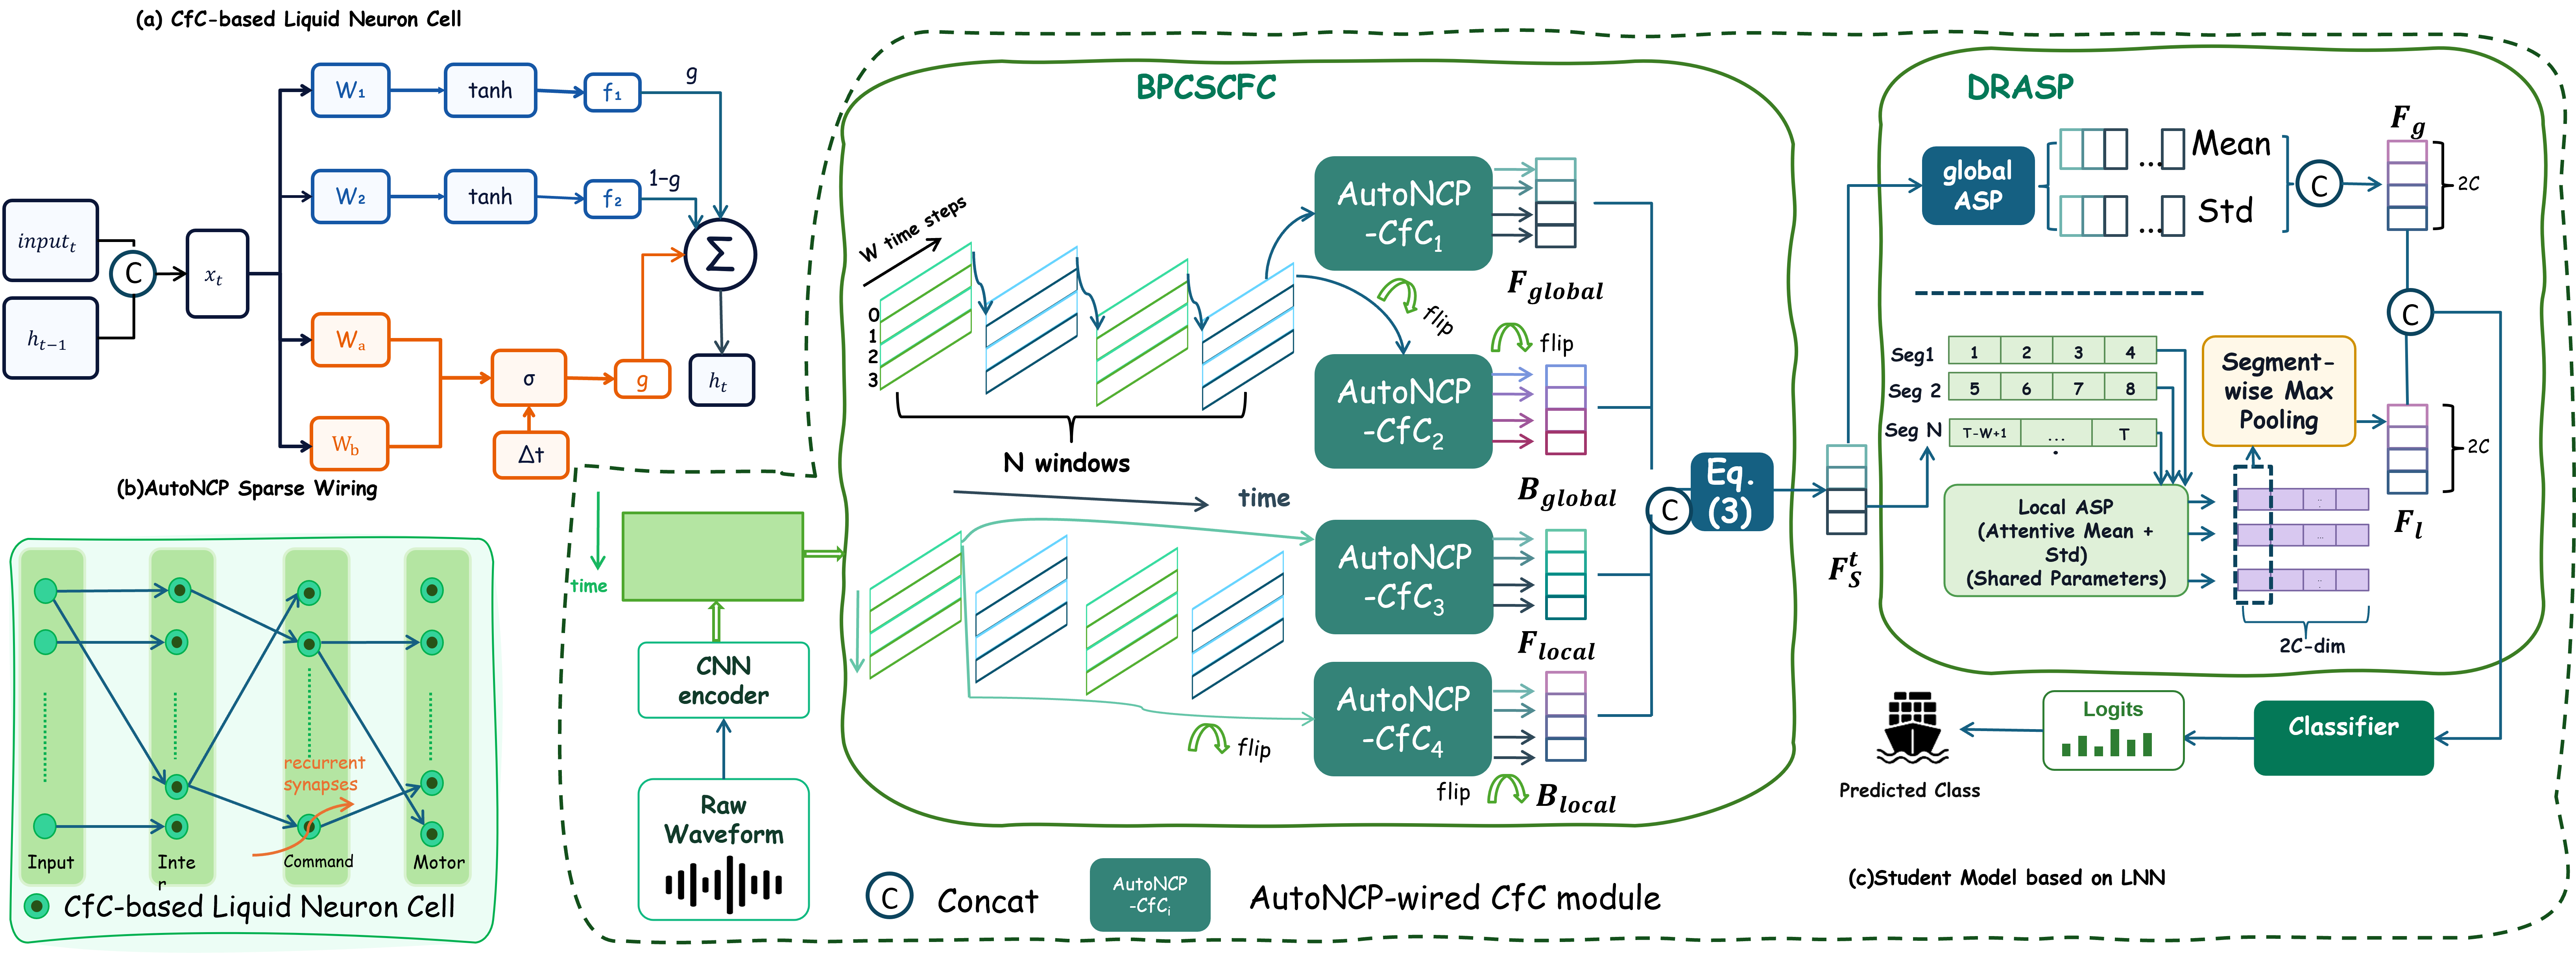
\includegraphics[width=\textwidth]{figures/Detailed Architecture of the Proposed Liquid Neural Student Network.png}
    \caption{Detailed architecture of the proposed liquid neural student network for underwater acoustic target recognition. A one-dimensional CNN encoder transforms the raw waveform into a temporal feature sequence, which is processed by the bidirectional parallel cross-slicing CfC (BPCSCfC) module with AutoNCP-wired CfC cells. The dual-resolution attentive statistics pooling (DRASP) module then combines global attentive statistics with segment-wise local attentive statistics to form the utterance-level representation used by the classifier.}
    \label{fig:student_architecture}
\end{figure*}

\begin{algorithm}[!t]
\caption{Student Network for Underwater Acoustic Recognition}
\label{alg:student_network}
\begin{algorithmic}[1]
\Require $\mathbf{s}\in\mathbb{R}^{B\times 1\times L}$; window length $W$ with $W\mid T_S$; class count $K$
\Ensure $\mathbf{H}_S,\mathbf{F}_S^t\in\mathbb{R}^{B\times T_S\times C}$
\Ensure $\mathbf{Z}_S^t\in\mathbb{R}^{B\times T_S\times K}$; $\mathbf{Z}_S\in\mathbb{R}^{B\times K}$
\State $\mathbf{H}_S \gets \operatorname{Transpose}_{C,T}\big(\operatorname{CNNEncoder}(\mathbf{s})\big)$
\State $N \gets T_S/W$
\State $(\mathbf{H}^{f},\mathbf{H}^{b}) \gets (\mathbf{H}_S,\operatorname{Reverse}_{T}(\mathbf{H}_S))$
\For{$d\in\{f,b\}$} \Comment{Forward and backward temporal directions}
    \State $\mathbf{X}^{d} \gets \operatorname{Reshape}(\mathbf{H}^{d},B,N,W,C)$
    \State $\tilde{\mathbf{X}}_{l}^{d} \gets \operatorname{Reshape}(\mathbf{X}^{d},B N,W,C)$
    \State $\tilde{\mathbf{X}}_{g}^{d} \gets \operatorname{Reshape}\big(\operatorname{Permute}_{N,W}(\mathbf{X}^{d}),B W,N,C\big)$
    \State $\mathbf{Y}_{l}^{d} \gets \operatorname{AutoNCP\mbox{-}CfC}_{l}^{d}(\tilde{\mathbf{X}}_{l}^{d})$ \Comment{Closed-form update in (\ref{eq:cfc_update})}
    \State $\mathbf{Y}_{g}^{d} \gets \operatorname{AutoNCP\mbox{-}CfC}_{g}^{d}(\tilde{\mathbf{X}}_{g}^{d})$
    \State $\mathbf{O}_{l}^{d} \gets \operatorname{Reshape}(\mathbf{Y}_{l}^{d},B,T_S,C)$
    \State $\mathbf{O}_{g}^{d} \gets \operatorname{Reshape}(\mathbf{Y}_{g}^{d},B,W,N,C)$
    \State $\mathbf{O}_{g}^{d} \gets \operatorname{Reshape}(\operatorname{Permute}_{W,N}(\mathbf{O}_{g}^{d}),B,T_S,C)$
\EndFor
\State $(F_{\mathrm{local}},F_{\mathrm{global}}) \gets (\mathbf{O}_{l}^{f},\mathbf{O}_{g}^{f})$
\State $B_{\mathrm{local}} \gets \operatorname{Reverse}_{T}(\mathbf{O}_{l}^{b})$
\State $B_{\mathrm{global}} \gets \operatorname{Reverse}_{T}(\mathbf{O}_{g}^{b})$
\State $\mathbf{U} \gets \operatorname{Concat}_{C}(F_{\mathrm{local}},F_{\mathrm{global}},B_{\mathrm{local}},B_{\mathrm{global}})$
\State $\mathbf{F}_S^t \gets \operatorname{G}\big(\operatorname{LN}(\mathbf{W}_{p}\mathbf{U}+\mathbf{b}_{p})\big)$
\State $\mathbf{Z}_S^t \gets \operatorname{Linear}_{\mathrm{temp}}(\mathbf{F}_S^t)$ \Comment{Used by TS-T during distillation}
\State $\mathbf{F}_g \gets \operatorname{GlobalASP}((\mathbf{F}_S^t)^\top)$
\State $\{\mathbf{F}_{S,m}^t\}_{m=1}^{M} \gets \operatorname{PadAndSegment}_{W}(\mathbf{F}_S^t)$
\For{$m=1$ to $M$}
    \State $\mathbf{F}_{l,m} \gets \operatorname{LocalASP}((\mathbf{F}_{S,m}^t)^\top)$ \Comment{Shared local-ASP parameters}
\EndFor
\State $\mathbf{F}_l \gets \operatorname{MaxPool}_{m}(\{\mathbf{F}_{l,m}\}_{m=1}^{M})$
\State $\mathbf{F}_{\mathrm{pooled}} \gets \operatorname{Concat}_{C}(\mathbf{F}_g,\mathbf{F}_l)$
\State $\mathbf{Z}_S \gets \operatorname{Classifier}(\mathbf{F}_{\mathrm{pooled}})$
\State \Return $\mathbf{Z}_S$, $\mathbf{Z}_S^t$, $\mathbf{F}_S^t$, $\mathbf{H}_S$ \Comment{$\mathbf{H}_S$ is used by MemKD}
\end{algorithmic}
\end{algorithm}

For local modeling, $\mathbf{H}_S$ is rearranged as $\mathbf{X}_l \in \mathbb{R}^{B \times N \times W \times C}$, where $N=T_S/W$ is the number of windows and $W$ is the window length. The batch and window dimensions are merged into $\tilde{\mathbf{X}}_l \in \mathbb{R}^{(B \cdot N) \times W \times C}$. The forward local stream models adjacent time steps inside each window to obtain $F_{\mathrm{local}}$. The backward local stream processes the time-reversed sequence and restores the original order to obtain $B_{\mathrm{local}}$. For global modeling, $\mathbf{H}_S$ is rearranged as $\mathbf{X}_g \in \mathbb{R}^{B \times W \times N \times C}$ and then transformed into $\tilde{\mathbf{X}}_g \in \mathbb{R}^{(B \cdot W) \times N \times C}$. The forward and backward global streams model cross-window dependencies to obtain $F_{\mathrm{global}}$ and $B_{\mathrm{global}}$. The four streams are concatenated along the channel dimension and passed through linear projection, layer normalization, and activation:
% \begin{equation}
% \mathbf{F}_S^t =
% \operatorname{G}
% \Big(
% \operatorname{LN}
% \big(
% \mathbf{W}\operatorname{Concat}(F_{\mathrm{local}},F_{\mathrm{global}},B_{\mathrm{local}},B_{\mathrm{global}})
% + \mathbf{b}
% \big)
% \Big),
% \quad
% \mathbf{F}_S^t \in \mathbb{R}^{B \times T_S \times C},
% \end{equation}
\begin{equation}
\begin{split}
    \mathbf{F}_S^t &= \operatorname{G} \Big( \operatorname{LN} \big( \mathbf{W}\cdot \operatorname{Concat} (F_{\mathrm{local}}, F_{\mathrm{global}}, \\
    &\quad B_{\mathrm{local}}, B_{\mathrm{global}}) + \mathbf{b} \big) \Big), 
\end{split}
\end{equation}
where$\quad \mathbf{F}_S^t \in \mathbb{R}^{B \times T_S \times C}$, $\operatorname{G}(\cdot)$ denotes the activation function, $\operatorname{LN}$ denotes layer normalization, and $\mathbf{W}$ and $\mathbf{b}$ are learnable parameters.
% 
Underwater acoustic signals contain both global acoustic characteristics, such as timbre and spectral energy distribution, and local transient events, such as mechanical start-up and burst noise. A single-scale pooling operation cannot capture both types of information. We therefore design DRASP with global and local branches. The global branch directly performs attentive statistics pooling on $\mathbf{F}_S^t$ after transposition to $\mathbf{F}\in \mathbb{R}^{B \times C \times T_S}$. The attention weight $\alpha \in \mathbb{R}^{B \times T_S}$ is computed as
\begin{equation}
\alpha = \operatorname{Softmax}_T \left( \mathbf{W}_{\alpha} \cdot \tanh(\mathbf{W}_{\beta} \cdot \mathbf{F}) \right),
\end{equation}
where $\mathbf{W}_{\alpha} \in \mathbb{R}^{1 \times C'}$ and $\mathbf{W}_{\beta} \in \mathbb{R}^{C' \times C}$ are learnable projection matrices. The weighted mean and standard deviation are then computed as
\begin{equation}
\mu = \sum_{t=1}^{T_S} \alpha_t \cdot \mathbf{F}_t, \quad
\sigma = \sqrt{ \sum_{t=1}^{T_S} \alpha_t \cdot (\mathbf{F}_t - \mu)^2 + \epsilon },
\end{equation}
where $\epsilon=10^{-6}$ is used for numerical stability. The global statistical feature is
\begin{equation}
\mathbf{F}_{g}=\operatorname{Concat}(\mu_g,\sigma_g) \in \mathbb{R}^{B \times 2C}.
\end{equation}
The local branch divides the input sequence into multiple short segments and applies attentive statistics pooling to each segment. The most salient local feature $\mathbf{F}_l \in \mathbb{R}^{B \times 2C}$ is selected by max pooling across segments. Finally, the global and local statistics are concatenated to obtain $\mathbf{F}_{\mathrm{pooled}} \in \mathbb{R}^{B \times 4C}$, which is fed to the classifier. This lightweight student network is suitable for underwater deployment and can inherit high-level semantic knowledge through distillation.

\subsection{Memory-Discrepancy Knowledge Distillation}
\label{subsec:memkd}
The intermediate sequence features of the student model are continuous hidden-state trajectories over time. For underwater acoustic signals with strong temporal correlation, directly aligning teacher and student feature maps is difficult because the two networks may have inconsistent feature distributions and dimensions. MemKD instead focuses on dynamic trajectory fitting. Short-term memory discrepancy captures instantaneous physical changes in acoustic signals, while long-term memory discrepancy mitigates the tendency to forget long-range dependencies. Thus, MemKD guides the LNN student to learn the teacher's temporal reasoning pattern across architectural differences.

The inputs of MemKD are intermediate features from the student and teacher models. Let $\mathbf{H}_S$ denote the student hidden state and $\mathbf{H}_T \in \mathbb{R}^{B \times T_t \times D_t}$ denote the corresponding teacher feature, where usually $T_t > T_S$ and $D_t \gg C$. We first use one-dimensional linear interpolation to align the teacher sequence length with the student:
\begin{equation}
\hat{\mathbf{H}}_T = \operatorname{Interp}(\mathbf{H}_{T}, T_S).
\end{equation}
For simplicity, $\hat{\mathbf{H}}_T$ is still denoted as $\mathbf{H}_T$ below.

Given a temporal offset $z$, the state variation of the teacher or student is
\begin{equation}
\Delta \mathbf{H}^t_{(\cdot)}
= \mathbf{H}^{t+z}_{(\cdot)} - \mathbf{H}^{t}_{(\cdot)},
\end{equation}
where $(\cdot)$ denotes either teacher or student. To reduce the influence of feature-scale differences, the difference vector is normalized by the current state norm:
\begin{equation}
\mathbf{F}^{(\cdot)}_t
= \frac{\Delta \mathbf{H}^t_{(\cdot)}}
{\|\mathbf{H}^t_{(\cdot)}\|_2 + \epsilon}.
\end{equation}
Because directional information is not directly comparable between heterogeneous networks, only the magnitude is retained:
\begin{equation}
\mathbf{M}^{(\cdot)}_t
= \left\|
\mathbf{F}^{(\cdot)}_t
\right\|_2.
\end{equation}
The memory trajectory is matched using Smooth L1 loss:
\begin{equation}
\mathcal{L}_{\mathrm{MemKD}}(z)
=
\frac{1}{T-z}
\sum_{t=1}^{T-z}
\mathrm{SmoothL1}
\Big(
\mathbf{M}^{S}_t,
\mathbf{M}^{T}_t
\Big).
\end{equation}

\paragraph{Short-term memory discrepancy}
When $z=1$, the short-term memory loss is
\begin{equation}
    \mathcal{L}_{\mathrm{s}}=\mathcal{L}_{\mathrm{MemKD}}(z=1),
\end{equation}
which captures local dynamic changes between adjacent frames.

\paragraph{Long-term memory discrepancy}
At each training step, a temporal offset is randomly sampled as
\(
z \sim \mathcal{U}\big(2,\lfloor T/2 \rfloor\big)
\).
The long-term memory loss is
\begin{equation}
    \mathcal{L}_{\mathrm{l}}=\mathcal{L}_{\mathrm{MemKD}}(z),
\end{equation}
which models stable dependencies across longer time spans. The final MemKD objective is
\begin{equation}
\mathcal{L}_{\mathrm{M}}
=
\lambda_s\, \mathcal{L}_{\mathrm{s}}
+
\lambda_l\, \mathcal{L}_{\mathrm{l}},
\end{equation}
where $\lambda_s$ and $\lambda_l$ are fixed hyperparameters balancing short-term transient cues and long-term temporal patterns.

\subsection{Temporal Separation with Adaptive Temperature Knowledge Distillation}
\label{subsec:tser}
Unlike conventional KD methods that align distributions only at the final output layer, TS-T constrains teacher and student semantic evolution trajectories along the time dimension. The teacher logits are denoted as $\mathbf{Z}_{T} \in \mathbb{R}^{B\times K}$. The student transforms $\mathbf{F}_S^t$ into time-step logits $\mathbf{Z}^{t}_S \in \mathbb{R}^{B \times T_s \times K}$, and its final classification logits are denoted as $\mathbf{Z}_S \in \mathbb{R}^{B \times K}$, where $K$ is the number of underwater acoustic categories.

The temperature coefficient is adaptively defined by the sample standard deviation of logits. Teacher and student logits are standardized by Z-score normalization. For an arbitrary logit vector $\mathbf{z}$,
\begin{equation}
\hat{z}_i = \frac{z_i - \mu_\mathbf{z}}{\sigma_\mathbf{z} + \epsilon},
\end{equation}
where $\mu_\mathbf{z}$ and $\sigma_\mathbf{z}$ are the mean and standard deviation over the class dimension, and $\epsilon$ prevents division by zero. In this formulation, $\sigma_\mathbf{z}$ acts as a parameter-free adaptive temperature that dynamically adjusts distribution smoothness.

To guide the student at every time step, $\mathbf{Z}_{T}$ is copied and broadcast along the temporal dimension to obtain $\mathbf{Z}_{T}^{t} \in \mathbb{R}^{B \times T_s \times K}$, which is aligned with $\mathbf{Z}_S^{t}$. The standardized teacher and student logits of the $i$-th sample at time step $t$ are denoted as $\hat{\mathbf{z}}_T^{(i,t)}$ and $\hat{\mathbf{z}}_S^{(i,t)}$. The sequential distillation loss is
\begin{equation}
\mathcal{L}_{\mathrm{TS\mbox{-}T}}^{\mathrm{seq}}
=
\frac{1}{B}
\sum_{i=1}^{B}
\sum_{t=1}^{T_s}
w_t
D_{\mathrm{KL}}
\left(
\sigma(\hat{\mathbf{z}}_{T}^{(i,t)})
\|
\sigma(\hat{\mathbf{z}}_{S}^{(i,t)})
\right),
\end{equation}
where $\sigma(\cdot)$ is the softmax function, $w_t$ is the temporal weight coefficient, and $D_{\mathrm{KL}}(\cdot)$ measures the distribution discrepancy at each time step. Uniform temporal weights are used in this work. To preserve consistency at the final decision layer, we further introduce
\begin{equation}
    \mathcal{L}_{\mathrm{TS\mbox{-}T}}^{\mathrm{final}}
    = D_{\mathrm{KL}}(Z_S \| Z_T).
\end{equation}
The TS-T objective is
\begin{equation}
\mathcal{L}_{\mathrm{TS\mbox{-}T}}
=
\beta \cdot \mathcal{L}_{\mathrm{TS\mbox{-}T}}^{\mathrm{seq}}
+
(1 - \beta)\cdot
\mathcal{L}_{\mathrm{TS\mbox{-}T}}^{\mathrm{final}},
\end{equation}
where $\beta$ is a learnable fusion coefficient. TS-T mainly constrains distribution consistency over time, while MemKD further learns hidden dynamic structures. These two components are complementary.

\subsection{Overall Training Loss}
\label{subsec:total_loss}
The overall framework in Fig.~\ref{fig:structure} follows the teacher--student paradigm. The student is based on the 
% closed-form-time
closed-form continuous-time LNN
LNN structure and performs downstream classification. The total training objective is
\begin{equation}
\mathcal{L}_{\mathrm{total}}
= \mathcal{L}_{\mathrm{CE}}
+ \lambda_m \, \mathcal{L}_{\mathrm{M}}
+ (1 - \lambda_m) \, \mathcal{L}_{\mathrm{TS\mbox{-}T}},
\end{equation}
where $\mathcal{L}_{\mathrm{CE}}$ is the standard cross-entropy classification loss of the student, and $\lambda_m$ balances the two distillation losses.

\section{Experiments}
\subsection{Experimental Setup}
\subsubsection{Benchmark Data Sets}
Two real-world ocean acoustic data sets are used: ShipsEar~\cite{David2016ShipsEar} and DeepShip~\cite{Irfan2021DeepShip}. ShipsEar contains five classes of underwater acoustic targets, including passenger ships, tugboats, cargo ships, background noise, and ocean biological sounds. It contains about 90 recordings with a total duration of more than four hours, collected along the Spanish coast at 52.7 kHz. DeepShip contains four classes of vessel radiated noise, including passenger ships, tankers, cargo ships, and roll-on/roll-off ships. It contains 265 recordings with a total duration of more than 47 hours, collected from different global sea areas at 32 kHz. For fair comparison, all audio signals are resampled to 16 kHz and cropped to a fixed length of 3 s. The data sets are divided into training, validation, and test sets at a ratio of 8:1:1. Details are shown in Table~\ref{tab:dataset}.

\begin{table}[htbp]
\centering
\caption{Configurations of DeepShip and ShipsEar Data Sets}
\label{tab:dataset}
% 1：调大行高，增加垂直呼吸感（非常关键！）
\renewcommand{\arraystretch}{1.1} 
% 2：微调列间距，找到最舒适的留白比例
\setlength{\tabcolsep}{10pt} 

% 3：@{} 去掉表格最左侧和最右侧的隐形空白，让顶线底线和文字完美齐平
\begin{tabular}{@{}lcc@{}} 
\toprule
Configurations & DeepShip & ShipsEar \\
\midrule
Dataset size & 53155 & 3738 \\
Category     & 4     & 5    \\
% 4：用 \makecell 精准换行，保持整体视觉重心居中
Location     & \makecell[c]{Canada Strait \\ of Georgia} & \makecell[c]{Spanish Atlantic \\ Coast} \\
Equipment    & \makecell[c]{icListen AF \\ Hydrophone}   & \makecell[c]{digitalHyd \\ SR-1} \\
\bottomrule
\end{tabular}
\end{table}

\subsubsection{Experimental Settings}
The entire model architecture was implemented using the PyTorch framework, and all experiments were conducted on an NVIDIA RTX 4090 GPU. The teacher model was a pretrained Wav2Vec 2.0-based audio classification network, whose parameters were frozen during the distillation process.
The distillation process was optimized using the AdamW optimizer with an initial learning rate of $5\times10^{-4}$, and the total number of training epochs was set to 200. The batch size was selected according to the characteristics and memory requirements of each dataset to ensure stable model convergence.
In the proposed TMSKD method, the memory difference calculation in the MemKD component incorporates both short-term and long-term losses, where the short-term offset is set to $z=1$ and the long-term offset is dynamically and randomly sampled from the range of $2$ to $8$. The weights of the short-term and long-term losses in MemKD are fixed to $\lambda_s=0.5$ and $\lambda_l=1.0$, respectively. In the TS-T component, temporal separation is performed with an adaptive temperature, and the learnable weight $\beta$ adaptively balances $\mathcal{L}_{\mathrm{TS\mbox{-}T}}^{\mathrm{seq}}$ and $\mathcal{L}_{\mathrm{TS\mbox{-}T}}^{\mathrm{final}}$.
The distillation objective combines the label loss and the soft distillation loss. A 10-fold cross-validation protocol was adopted to evaluate the model performance. Specifically, each dataset was randomly divided into 10 mutually exclusive subsets. In each round, one subset was used as the validation set and the remaining nine subsets were used as the training set. The final performance was reported as the average over the 10 experimental runs.

\subsubsection{Evaluation Metrics}
We evaluate recognition performance using accuracy (ACC), F1-score, and area under the curve (AUC). ACC measures the proportion of correctly classified samples. F1-score accounts for class imbalance by balancing precision and recall, while AUC evaluates classification ability under different thresholds. To assess deployment efficiency, we further analyze parameter count, floating-point operations (FLOPs), model size, and inference latency~\cite{Han2016DeepCompression}. These metrics provide a comprehensive evaluation of TMSKD in terms of accuracy, efficiency, and robustness.

\subsection{Comparison Experiments}
\subsubsection{Comparison With State-of-the-Art KD Methods}
The proposed TMSKD is compared with 21 classical or popular state-of-the-art KD methods, including logits-based methods such as KD~\cite{Hinton2015Distilling}, DKD~\cite{Zhao2022DKD}, NKD~\cite{Yang2023NKD}, LSKD~\cite{Sun2024LSKD}, SDD~\cite{Wei2024SDD}, and WSLD~\cite{Zhou2021WSLD}, as well as feature-based methods such as AT~\cite{Zagoruyko2017AT}, SP~\cite{Tung2019SP}, FSP~\cite{Yim2017FSP}, NST~\cite{Huang2017NST}, RKD~\cite{Park2019RKD}, PKT~\cite{Passalis2018PKT}, MGD~\cite{Yang2022MGD}, and MKD~\cite{Lao2023MKD}.

As shown in Table~\ref{tab:distillation_results}, TMSKD achieves the best performance on both data sets across ACC, F1-score, and AUC. On DeepShip, TMSKD reaches 93.41\%, 93.40\%, and 99.17\% in ACC, F1-score, and AUC, respectively, improving over the second-best method by 0.85, 0.87, and 0.10 percentage points. On ShipsEar, TMSKD reaches 92.39\%, 92.34\%, and 98.84\%, improving over the second-best method by 2.36, 2.96, and 0.53 percentage points. Compared with the non-distilled student, TMSKD improves ACC, F1-score, and AUC by 5.67, 5.68, and 1.47 percentage points on DeepShip and by 4.14, 4.35, and 1.01 percentage points on ShipsEar. These results show that the proposed method effectively compensates for the performance gap of the lightweight student.
\begin{table*}[!htbp]
\centering
\caption{Performance Comparison of Different Distillation Methods on DeepShip and ShipsEar Data Sets. Top three results are colored in \textcolor{red}{red}, \textcolor{blue}{blue}, and \textcolor{green}{green}, respectively.
$\uparrow$ indicates the improvement of TMSKD over the second-best method.
$\uparrow\uparrow$ denotes the improvement of TMSKD over the student model.}
\label{tab:distillation_results}
\small
\setlength{\tabcolsep}{4pt}
\begin{tabular}{c|c|c|c|c|c|c|c}
\toprule
\multirow{2}{*}{Distillation Mechanism} &
\multirow{2}{*}{Method} &
\multicolumn{3}{c|}{DeepShip} &
\multicolumn{3}{c}{ShipsEar} \\
& & ACC & F1-score & AUC & ACC & F1-score & AUC \\
\midrule
\multirow{2}{*}{\makecell{Baseline \\ (No KD)}}
& Teacher (wav2vec 2.0) & 98.56 & 98.56 & 99.93 & 94.66 & 94.66 & 99.63 \\
& Student (LNN) & 83.74 & 87.72 & 97.70 & 86.44 & 87.99 & 97.83 \\
\midrule
\multirow{6}{*}{Logits}
& KD~\cite{Hinton2015Distilling}  & 91.86 & 91.83 & 99.03 & \textcolor{blue}{90.03} & \textcolor{blue}{89.38} & 98.27 \\
& DKD~\cite{Zhao2022DKD} & \textcolor{green}{92.12} & \textcolor{green}{92.08} & 98.94 & 88.70 & 87.78 & 97.78 \\
& NKD~\cite{Yang2023NKD} & 91.75 & 91.72 & 98.91 & 89.10 & 87.73 & 98.09 \\
& LSKD~\cite{Sun2024LSKD} & 91.35 & 91.32 & 98.89 & 89.10 & 88.71 & 98.21 \\
& SDD~\cite{Wei2024SDD} & 91.23 & 91.19 & 98.79 & 89.10 & 88.38 & \textcolor{green}{98.28} \\
& WSLD~\cite{Zhou2021WSLD} & 91.37 & 91.32 & 98.89 & 88.43 & 87.89 & 98.12 \\
\midrule
\multirow{15}{*}{Feature}
& AT~\cite{Zagoruyko2017AT} & 90.80 & 90.77 & 98.76 & 89.49 & \textcolor{green}{88.98} & 98.02 \\
& SP~\cite{Tung2019SP} & 91.26 & 91.22 & 98.88 & 88.30 & 87.88 & 98.06 \\
& FSP~\cite{Yim2017FSP} & \textcolor{blue}{92.56} & \textcolor{blue}{92.53} & \textcolor{blue}{99.07} & 88.43 & 86.86 & 97.62 \\
& NST~\cite{Huang2017NST} & 90.72 & 90.69 & 98.89 & 87.50 & 86.87 & 97.71 \\
& RKD~\cite{Park2019RKD} & 91.32 & 91.28 & 98.95 & 87.77 & 86.55 & 97.38 \\
& PKT~\cite{Passalis2018PKT} & 89.47 & 89.42 & 98.62 & 88.56 & 87.33 & 97.92 \\
& FreeKD~\cite{Zhang2024FreeKD} & 91.68 & 91.63 & 98.90 & 87.23 & 86.33 & 97.81 \\
& CC~\cite{Peng2019CC} & 91.20 & 91.16 & 98.87 & 88.96 & 88.22 & 98.08 \\
& VID~\cite{Ahn2019VID} & 91.20 & 91.15 & 98.84 & 88.30 & 87.75 & 98.08 \\
& VKD~\cite{Miles2024VKD} & 89.47 & 89.40 & 98.51 & 87.77 & 86.93 & 97.67 \\
& MGD~\cite{Yang2022MGD} & 91.12 & 91.09 & 98.90 & 88.43 & 87.73 & 97.94 \\
& DiffKD~\cite{Huang2023DiffKD} & 89.04 & 88.98 & 98.44 & 88.56 & 87.95 & 98.07 \\
& MKD~\cite{Lao2023MKD} & 92.02 & 91.99 & \textcolor{green}{99.04} & \textcolor{green}{89.36} & 88.71 & \textcolor{blue}{98.31} \\
& CAT-KD~\cite{Guo2023CATKD} & 89.40 & 89.33 & 98.49 & 87.63 & 86.65 & 97.92 \\
& ICKD~\cite{Liu2021ICKD} & 91.24 & 91.18 & 98.96 & 84.71 & 83.81 & 97.22 \\
\midrule
\rowcolor{gray!15}
& \textbf{TMSKD (Ours)} &
\textcolor{red}{93.41} &
\textcolor{red}{93.40} &
\textcolor{red}{99.17} &
\textcolor{red}{92.39} &
\textcolor{red}{92.34} &
\textcolor{red}{98.84} \\
& $\uparrow$ & \textbf{+0.85} & \textbf{+0.87} & \textbf{+0.10} & \textbf{+2.36} & \textbf{+2.96} & \textbf{+0.53} \\
& $\Uparrow$ & \textbf{+9.67} & \textbf{+5.68} & \textbf{+1.47} & \textbf{+5.95} & \textbf{+4.35} & \textbf{+1.01} \\
\bottomrule
\end{tabular}
% \vspace{0.2mm}
\end{table*}


\subsubsection{Comparison With State-of-the-Art UATR Methods}
Table~\ref{tab:comparison with Different UATR Methods} compares the recognition accuracy and model complexity of the proposed method with representative UATR methods. Among the three newly included visual backbones, MobileViT-XXS achieved the highest DeepShip ACC of 96.61\% with CQT input. This result exceeded the 93.41\% obtained by the TMSKD-distilled LNN-3 by 3.20 percentage points. On ShipsEar, T-F Token ViT achieved the highest overall ACC of 98.15\%. Among the three visual backbones, MobileOne S0 achieved the best ShipsEar ACC of 96.26\% with Mel-spectrogram input, exceeding LNN-3 by 3.87 percentage points. Thus, the spectrogram-based models retained an accuracy advantage, whereas LNN-3 achieved 93.41\% and 92.39\% ACC by directly processing raw waveforms.

\begin{table*}[!htbp]
\centering
\caption{Performance Comparison With Different UATR Methods on DeepShip and ShipsEar Data Sets. For MobileOne S0, GhostNet V2 1$\times$, and MobileViT-XXS, ACC values are reported in the order Mel/CQT. Bold font indicates the best results.}
\label{tab:comparison with Different UATR Methods}
\small
\setlength{\tabcolsep}{4pt}
\begin{tabular}{c|c|c|c|c|c|c}
\toprule
\multirow{2}{*}{Method} &
\multicolumn{1}{c|}{Model} &
\multicolumn{1}{c|}{Model Size} &
\multicolumn{1}{c|}{FLOPs} &
\multicolumn{1}{c|}{Latency} &
\multicolumn{1}{c|}{DeepShip} &
\multicolumn{1}{c}{ShipsEar} \\
 & Parameters (M) & (MB) & (MFLOPS) & (ms) & ACC & ACC \\
\midrule
ALSI~\cite{ALSIUATR} & 28.34 & 109.21 & 3344.40 & 7.66 & 84.14 & 97.89  \\
MHT-UATR~\cite{MHTUATR} & 5.52 & 23.07 & 911.00 & \textbf{2.76} & 81.75 & 96.15 \\
CAF-JT~\cite{CAFJTUATR} & 14.83 & 73.14 & 1770.36 & 4.31 & 83.86 & 97.65 \\
T-F Token ViT~\cite{TFTokenViT} & 24.78 & 95.54 & 2819.86 & 7.18 & 84.25 & \textbf{98.15} \\
MobileOne S0~\cite{Vasu2023MobileOne} & 5.2929 & -- & 1085.15 & 30.43 & 95.15 / 95.90 & 96.26 / 95.99 \\
GhostNet V2 1$\times$~\cite{Tang2022GhostNetV2} & 4.8810 & -- & 180.97 & 22.81 & 93.68 / 94.17 & 95.06 / 95.86 \\
MobileViT-XXS~\cite{Mehta2022MobileViT} & 1.0128 & -- & 1383.35 & 14.18 & 95.55 / \textbf{96.61} & 94.66 / 93.72 \\
\textbf{LNN (w/ KD)} & \textbf{0.32} & \textbf{1.21} & \textbf{58.97} & 12.16 & 93.41 & 92.39 \\
\bottomrule
\end{tabular}
% \vspace{2mm}
\end{table*}

LNN-3 showed a clear advantage in model complexity. It required only 0.32 M parameters and 58.97 MFLOPS, the lowest values among all compared methods. Relative to MobileViT-XXS, the smallest of the three visual backbones, LNN-3 reduced the parameter count and FLOPs by 68.40\% and 95.74\%, respectively. It also reduced inference latency from 14.18 ms to 12.16 ms. Even compared with GhostNet V2 1$\times$, which had the lowest computational cost among the three visual backbones, LNN-3 used 67.41\% fewer FLOPs. Moreover, LNN-3 accepted raw waveforms without Mel-spectrogram or CQT conversion. Because the table reports model FLOPs only, the computational cost of this spectral preprocessing is not included in the comparison. The model sizes of the three visual backbones were unavailable in the source comparison and are therefore denoted by ``--''. These results identify LNN-3 as a lower-complexity alternative when a moderate accuracy reduction is acceptable for raw-waveform and resource-constrained deployment.

% =========================================================
% Overall Ablation Study（表4）
% default: TS-T=true, MemKD=true
% =========================================================
\begin{table}[htbp]
\centering
\small
\caption{Overall Ablation Study of Different KD Components of TMSKD on DeepShip and ShipsEar Data Sets}
\label{tab:ablation}
\setlength{\tabcolsep}{10pt}
\begin{tabular}{c|c|c|c}
\toprule
TS-T & MemKD  & DeepShip ACC & ShipsEar ACC \\
\midrule
    &      & 83.74 & 86.44 \\
$\checkmark$ &     &86.93 & 88.30 \\
 & $\checkmark$ &84.85 & 89.63 \\
$\checkmark$ & $\checkmark$ & \textbf{93.41} & \textbf{92.39} \\
\bottomrule
\end{tabular}
\vspace{2mm}
\begin{flushleft}
\footnotesize
TS-T and MemKD denote temporal separation with adaptive temperature KD and memory-discrepancy KD, respectively.
\end{flushleft}
\end{table}




% % ==================== 第一段分析：ShipsEar ====================

% As illustrated in Fig.~\ref{fig:tsne_four_methods_logits_shipsear}, we visualize the feature distributions on the ShipsEar dataset using t-SNE. Because this dataset contains five distinct classes of acoustic signals, the feature space is inherently complex. The non-distilled student baseline (Fig.~\ref{fig:tsne_four_methods_logits_shipsear}a) exhibits clear class mixing, particularly in the central region where boundaries are blurred. While Logits KD (Fig.~\ref{fig:tsne_four_methods_logits_shipsear}b) and Feature KD (Fig.~\ref{fig:tsne_four_methods_logits_shipsear}c) enhance the overall clustering tendency, local overlaps remain prevalent. Conversely, the proposed TMSKD framework (Fig.~\ref{fig:tsne_four_methods_logits_shipsear}d) yields highly distinct spatial partitions, significantly reducing category crossing in the transition regions. These visualization results are highly consistent with our quantitative evaluations, further validating the effectiveness of TMSKD in learning discriminative representations.

% % ==================== Fig 3：ShipsEar (单栏 2x2 结构) ====================
% \begin{figure}[!t] % 去掉星号，改为单栏环境
%     \centering
%     % ---- 第一排：(a) 和 (b) ----
%     \begin{minipage}[t]{0.48\linewidth} % 宽度必须改用 \linewidth 或 \columnwidth
%         \centering
%         
\includegraphics[width=\linewidth]{figures/tsne_four_methods_shipsear_v2/tsne_baseline_logits_single_column.png}
%         \par\footnotesize (a) Student baseline
%     \end{minipage}\hfill
%     \begin{minipage}[t]{0.48\linewidth}
%         \centering
%         
\includegraphics[width=\linewidth]{figures/tsne_four_methods_shipsear_v2/tsne_logits_kd_logits_single_column.png}
%         \par\footnotesize (b) Logits KD
%     \end{minipage}

%     \vspace{0.5em} % 单栏空间较小，上下排间距微调为 0.5em，显得更紧凑

%     % ---- 第二排：(c) 和 (d) ----
%     \begin{minipage}[t]{0.48\linewidth}
%         \centering
%         
\includegraphics[width=\linewidth]{figures/tsne_four_methods_shipsear_v2/tsne_feature_kd_logits_single_column.png}
%         \par\footnotesize (c) Feature KD
%     \end{minipage}\hfill
%     \begin{minipage}[t]{0.48\linewidth}
%         \centering
%         
\includegraphics[width=\linewidth]{figures/tsne_four_methods_shipsear_v2/tsne_best_logits_single_column.png}
%         \par\footnotesize (d) TMSKD
%     \end{minipage}

%     \caption{Four-method t-SNE comparison of logits on the ShipsEar dataset.}
%     \label{fig:tsne_four_methods_logits_shipsear}
% \end{figure}


% % ==================== 第二段分析：DeepShip ====================
% Furthermore, Fig.~\ref{fig:tsne_four_methods_logits_deepship} presents the t-SNE visualizations on the DeepShip dataset. The baseline student model (Fig.~\ref{fig:tsne_four_methods_logits_deepship}a) forms an initial category distribution, yet distinct classes still heavily overlap in the central feature space and near cluster boundaries. Although Logits KD (Fig.~\ref{fig:tsne_four_methods_logits_deepship}b) improves the clustering structure to some extent, local class adjacency and crossing persist. Feature KD (Fig.~\ref{fig:tsne_four_methods_logits_deepship}c) enhances the separation of certain clusters, but mixed samples are still observable in the transition regions. In sharp contrast, TMSKD (Fig.~\ref{fig:tsne_four_methods_logits_deepship}d) produces a remarkably clear four-class distribution with stronger intra-class compactness and larger inter-class margins. This demonstrates that TMSKD substantially improves the discriminative capability of the student network's output representations.


% \begin{figure}[!t] % 1. 去掉星号，改为单栏环境
%     \centering
%     % ---- 第一排：(a) 和 (b) ----
%     \begin{minipage}[t]{0.48\linewidth} % 2. 宽度限制在当前栏宽 (\linewidth)
%         \centering
%         
\includegraphics[width=\linewidth]{figures/tsne_four_methods_deepship_v2/tsne_baseline_logits_single_column.png}
%         \par\footnotesize (a) Student baseline % 3. 字体缩小为 \footnotesize 防折行
%     \end{minipage}\hfill
%     \begin{minipage}[t]{0.48\linewidth}
%         \centering
%         
\includegraphics[width=\linewidth]{figures/tsne_four_methods_deepship_v2/tsne_logits_kd_logits_single_column.png}
%         \par\footnotesize (b) Logits KD
%     \end{minipage}

%     \vspace{0.5em} % 单栏空间较小，上下排间距微调为 0.5em，显得更紧凑

%     % ---- 第二排：(c) 和 (d) ----
%     \begin{minipage}[t]{0.48\linewidth}
%         \centering
%         
\includegraphics[width=\linewidth]{figures/tsne_four_methods_deepship_v2/tsne_feature_kd_logits_single_column.png}
%         \par\footnotesize (c) Feature KD
%     \end{minipage}\hfill
%     \begin{minipage}[t]{0.48\linewidth}
%         \centering
%         
\includegraphics[width=\linewidth]{figures/tsne_four_methods_deepship_v2/tsne_best_logits_single_column.png}
%         \par\footnotesize (d) TMSKD
%     \end{minipage}

%     \caption{Four-method t-SNE comparison of logits on the DeepShip dataset.}
%     \label{fig:tsne_four_methods_logits_deepship}
% \end{figure}

% ==================== Fig 4：DeepShip (2x2 排版) ====================
% \begin{figure*}[!t]
%     \centering
%     % ---- 第一排：(a) 和 (b) ----
%     \begin{minipage}[t]{0.48\textwidth}
%         \centering
%         
\includegraphics[width=\linewidth]{figures/tsne_four_methods_deepship_v2/tsne_baseline_logits_single_column.png}
%         \par\small (a) Student baseline
%     \end{minipage}\hfill
%     \begin{minipage}[t]{0.48\textwidth}
%         \centering
%         
\includegraphics[width=\linewidth]{figures/tsne_four_methods_deepship_v2/tsne_logits_kd_logits_single_column.png}
%         \par\small (b) Logits KD
%     \end{minipage}

%     \vspace{1em} % 两排之间的垂直间距

%     % ---- 第二排：(c) 和 (d) ----
%     \begin{minipage}[t]{0.48\textwidth}
%         \centering
%         
\includegraphics[width=\linewidth]{figures/tsne_four_methods_deepship_v2/tsne_feature_kd_logits_single_column.png}
%         \par\small (c) Feature KD
%     \end{minipage}\hfill
%     \begin{minipage}[t]{0.48\textwidth}
%         \centering
%         
\includegraphics[width=\linewidth]{figures/tsne_four_methods_deepship_v2/tsne_best_logits_single_column.png}
%         \par\small (d) TMSKD
%     \end{minipage}

%     \caption{Four-method t-SNE comparison of logits on the DeepShip dataset.}
%     \label{fig:tsne_four_methods_logits_deepship}
% \end{figure*}
\subsection{Ablation Study and Hyperparameter Analysis}

To verify the effectiveness of the key distillation components in TMSKD, we conduct systematic ablation experiments on DeepShip and ShipsEar. As shown in Table~\ref{tab:ablation}, without any distillation strategy, the baseline model achieves 83.74\% and 86.44\% ACC on DeepShip and ShipsEar, respectively. When only TS-T is introduced, the model reaches 86.93\% and 88.30\%, indicating that adaptive-temperature temporal separation can transfer inter-class relations from the output distribution level, but cannot fully describe dynamic temporal structures alone. When only MemKD is used, the model reaches 84.85\% and 89.63\%, showing that memory-discrepancy distillation effectively captures temporal dynamic structure. When TS-T and MemKD are combined, the model achieves 93.41\% and 92.39\%, substantially improving over the baseline. This demonstrates the complementarity of the two strategies.

We further analyze the effects of the TS-T fusion coefficient, MemKD memory constraints, temporal offset ranges, and student architecture parameters. The following results show that different hyperparameters affect model performance, while most settings around the default configuration remain competitive, indicating the stability of the proposed framework.
Table~\ref{tab:beta_analysis} evaluates the initialization of the learnable TS-T fusion coefficient $\beta$. On DeepShip, all initial values produce high ACC values from 93.03\% to 93.41\%, and the default initialization of 0.5 gives the best result. On ShipsEar, the same initialization achieves the complete TMSKD result of 92.39\%, while the other initializations remain lower but still stable. These results indicate that the learnable fusion coefficient is not overly sensitive to its initialization, and that the default setting provides a robust balance between time-step sequential distillation and final-logit distillation.


% =========================================================
% 01. Beta Analysis（表5）
% default: learnable_beta=true, beta initialization=0.5
% =========================================================
\begin{table}[htbp]
\centering
\caption{Performance Evaluation of the Learnable Coefficient $\beta$}
\label{tab:beta_analysis}
\small
\setlength{\tabcolsep}{10pt}
\begin{tabular}{c|c|c}
\toprule
\makecell{Learnable $\beta$\\Initialization} &
\makecell{DeepShip\\ACC} &
\makecell{ShipsEar\\ACC} \\
\midrule
0.1 & 93.03 & 89.23 \\
% 93.03来自checkpoints/hyperparameter_analysis/01_beta_analysis/B1_learnable_beta_init_0_1/train_20260530_130732.log Epoch [195/200]
0.3 & 93.12 & 90.03 \\
% 93.12来自checkpoints/hyperparameter_analysis/01_beta_analysis/B2_learnable_beta_init_0_3/train_20260530_220629.log Epoch [197/200]
\rowcolor{gray!15}
0.5(Default) & \textbf{93.41} & \textbf{92.39} \\
0.7 & 93.24 & 90.03 \\
0.9 & 93.17 & 90.56 \\
% \rowcolor{gray!15} 终于改掉了！原来是这个地方
% \textbf{Default} & 93.41 & 92.39 \\
\bottomrule
\end{tabular}
\vspace{0.5ex}
\par\footnotesize $\beta$ is the learnable fusion coefficient in the TS-T objective, balancing the time-step sequential distillation loss and the final-logit distillation loss; the listed value is its initialization, and the gray row is the default setting.
\end{table}

% =========================================================
% 03. MemKD Short-/Long-Term Weight Analysis（表6）
% default: lambda_s=0.5, lambda_l=1.0
% =========================================================
Table~\ref{tab:memkd_weight_analysis} analyzes the short- and long-term weights in MemKD. The default setting of $\lambda_s=0.50$ and $\lambda_l=1.0$ achieves the highest ACC on both DeepShip and ShipsEar, reaching 93.41\% and 92.39\%, respectively. Other weight combinations remain competitive on DeepShip but lead to more evident degradation on ShipsEar, indicating that an appropriate balance between short-term local changes and long-term temporal evolution is important for robust cross-data-set performance.

\begin{table}[htbp]
\centering
\caption{Performance evaluation of the short- and long-term weights in MemKD.}
\label{tab:memkd_weight_analysis}
\small
\setlength{\tabcolsep}{9pt}
\begin{tabular}{c|c|c|c}
\toprule
$\lambda_s$ & $\lambda_l$ &
\makecell{DeepShip\\ACC} &
\makecell{ShipsEar\\ACC} \\
\midrule
0.25 & 0.5 & 93.05 & 89.49 \\
% 93.05 来自于checkpoints/hyperparameter_analysis/03_memkd_weight_analysis/M1_short_0_25_long_0_5/train_20260524_155203.log Epoch [196/200]
0.25 & 1.0 & 93.17 & 89.23 \\
% 93.17 来自于checkpoints/hyperparameter_analysis/03_memkd_weight_analysis/M2_short_0_25_long_1_0/train_20260525_044341.log Epoch [194/200]
0.25 & 2.0 & 93.02 & 89.76 \\
% 93.02 来自于checkpoints/hyperparameter_analysis/03_memkd_weight_analysis/M3_short_0_25_long_2_0/train_20260525_180604.log Epoch [200/200]
0.50 & 0.5 & 93.16 & 89.49 \\
\rowcolor{gray!15}
\textbf{0.50} & \textbf{1.0} & 93.41 & 92.39 \\
0.50 & 2.0 & 93.07 & 89.89 \\
% 93.07 来自于checkpoints/hyperparameter_analysis/03_memkd_weight_analysis/M6_short_0_5_long_2_0/train_20260527_045704.log Epoch [200/200]
1.00 & 0.5 & 93.18 & 91.22 \\
% 93.18 来自于checkpoints/hyperparameter_analysis/03_memkd_weight_analysis/M7_short_1_0_long_0_5/train_20260527_155242.log Epoch [194/200]
1.00 & 1.0 & 93.13 & 90.16 \\
% 93.13 来自于checkpoints/hyperparameter_analysis/03_memkd_weight_analysis/M8_short_1_0_long_1_0/train_20260528_031802.log Epoch [197/200]
1.00 & 2.0 & 93.12 & 90.82 \\
% 93.12 来自于checkpoints/hyperparameter_analysis/03_memkd_weight_analysis/M9_short_1_0_long_2_0/train_20260528_120848.log Epoch [200/200]
\bottomrule
\end{tabular}
\vspace{0.5ex}
\par\footnotesize $\lambda_s$ and $\lambda_l$ correspond to the short-term loss $\mathcal{L}_{\mathrm{s}}$ and long-term loss $\mathcal{L}_{\mathrm{l}}$ in the MemKD objective, respectively; the gray row is the default setting.
\end{table}

% \begin{table}[htbp]
% \centering
% \caption{Performance Evaluation of the Short- and Long-Term Weights in MemKD}
% \label{tab:memkd_weight_analysis}
% \small
% \setlength{\tabcolsep}{9pt}
% \begin{tabular}{c|c|c|c}
% \toprule
% $\lambda_s$ & $\lambda_l$ &
% \makecell{DeepShip\\ACC} &
% \makecell{ShipsEar\\ACC} \\
% \midrule
% 0.25 & 0.5 & 93.63 & 89.49 \\
% 0.25 & 1.0 & \textbf{94.41} & 89.23 \\
% 0.25 & 2.0 & 93.66 & 89.76 \\
% 0.50 & 0.5 & 93.16 & 89.49 \\
% \rowcolor{gray!15}
% \textbf{0.50} & \textbf{1.0} & 93.47 & 90.29 \\
% 0.50 & 2.0 & 93.47 & 89.89 \\
% 1.00 & 0.5 & 93.55 & \textbf{91.22} \\
% 1.00 & 1.0 & 93.93 & 90.16 \\
% 1.00 & 2.0 & 93.60 & 90.82 \\
% \bottomrule
% \end{tabular}
% \end{table}

Table~\ref{tab:z_random_range_analysis} reports the influence of the long-term temporal offset range $z$ in MemKD. The default \texttt{half} range achieves the best results on both DeepShip and ShipsEar, reaching 93.41\% and 92.39\%, respectively. In contrast, the \texttt{quarter} range reduces the temporal span available for long-term discrepancy modeling, while \texttt{upper\_half} biases the sampling toward more distant offsets and brings lower accuracy, especially on ShipsEar. This trend suggests that a moderate offset range provides a more reliable trade-off between capturing long-range dynamics and avoiding weakly related temporal noise.

% =========================================================
% 04. z_random Range Analysis（表7）
% default: z_random_range=half
% =========================================================
\begin{table}[htbp]
\centering
\small
\caption{Performance Evaluation of the Long-Term Temporal Offset Range in MemKD}
\label{tab:z_random_range_analysis}
\renewcommand{\arraystretch}{1.2}

\begin{tabular}{
>{\centering\arraybackslash}m{0.30\columnwidth}|
>{\centering\arraybackslash}m{0.22\columnwidth}|
>{\centering\arraybackslash}m{0.22\columnwidth}
}
\toprule
\makecell[c]{Long-Term Offset\\Range of $z$}
&
\makecell[c]{DeepShip\\ACC}
&
\makecell[c]{ShipsEar\\ACC}
\\
\midrule

\texttt{quarter}
& 92.93
& 90.43
\\

\rowcolor{gray!15}
\textbf{\texttt{half}}
& \textbf{93.41}
& \textbf{92.39}
\\

\texttt{upper\_half}
& 93.15
& 90.96
\\

\bottomrule
\end{tabular}

\vspace{0.5ex}
\par\footnotesize
$z$ is the temporal offset in
$\Delta \mathbf{H}^{t}_{(\cdot)}
=
\mathbf{H}^{t+z}_{(\cdot)}
-
\mathbf{H}^{t}_{(\cdot)}$
and is used to construct the long-term MemKD discrepancy;
\texttt{quarter}, \texttt{half}, and \texttt{upper\_half}
correspond to different sampling ranges within the sequence.
\end{table}
% =========================================================
% 05. BPCSCfC Branch Ablation（表8）
% default: cfc_branch_mode=full
% =========================================================
Table~\ref{tab:cfc_branch_analysis} verifies the contribution of different BPCSCfC branches. Using only the forward local branch provides a reasonable baseline, and adding the forward global branch further improves ShipsEar performance. However, the full branch configuration achieves the highest DeepShip ACC and the complete TMSKD result on ShipsEar. This confirms that bidirectional temporal modeling and the combination of local and global information improve the representation capability of the LNN student.

\begin{table}[htbp]
\centering
\small
\caption{Performance Evaluation of the BPCSCfC Branch Configuration}
\label{tab:cfc_branch_analysis}
\renewcommand{\arraystretch}{1.2}

\begin{tabular}{c|c|c|c|c|c}
\toprule
FL & FG & BL & BG & DeepShip ACC & ShipsEar ACC \\
\midrule
$\checkmark$ &              &              &              & 92.82 & 90.56 \\
$\checkmark$ & $\checkmark$ &              &              & 93.31 & 90.69 \\
$\checkmark$ &              & $\checkmark$ &              & 93.09 & 90.29 \\

\rowcolor{gray!15}
$\checkmark$ & $\checkmark$ & $\checkmark$ & $\checkmark$
& \textbf{93.41} & \textbf{92.39} \\

\bottomrule
\end{tabular}

\vspace{0.5ex}
\par\footnotesize
FL, FG, BL, and BG correspond to
$F_{\mathrm{local}}$, $F_{\mathrm{global}}$,
$B_{\mathrm{local}}$, and $B_{\mathrm{global}}$
in BPCSCfC, respectively; the gray row is the default
full-branch configuration.
\end{table}

% =========================================================
% 06. Temporal Granularity Analysis（表9）
% default: window_size=4, drasp_segment_len=4
% =========================================================
Table~\ref{tab:temporal_granularity_analysis} studies the window and segment length used for temporal partitioning. The default 4/4 setting obtains the best ACC on both DeepShip and ShipsEar, reaching 93.41\% and 92.39\%, respectively. Shorter granularities such as 1/1 and 2/2 may preserve fine local details but provide weaker sequence-level aggregation, whereas larger granularities such as 8/8 and 16/16 can reduce temporal resolution. These results show that the 4/4 setting provides a practical balance between local temporal sensitivity and robust sequence-level representation.

\begin{table}[htbp]
\centering
\caption{Performance Evaluation of the Temporal Granularity}
\label{tab:temporal_granularity_analysis}
\small
\setlength{\tabcolsep}{10pt}
\begin{tabular}{c|c|c}
\toprule
\makecell{Window/Segment\\Length} &
\makecell{DeepShip\\ACC} &
\makecell{ShipsEar\\ACC} \\
\midrule
1/1   & 91.15 & 91.36 \\
2/2   & 91.85 & 89.89 \\
\rowcolor{gray!15}
\textbf{4/4} & \textbf{93.41} & 92.39 \\
8/8   & 93.02 & 89.23 \\
16/16 & 91.46 & 90.56 \\
\bottomrule
\end{tabular}
\vspace{0.5ex}
\par\footnotesize Window/segment length corresponds to the BPCSCfC window length $W$ and the local DRASP segment length, controlling the temporal granularity for sequence partitioning and pooling; the gray row is the default setting.
\end{table}

% =========================================================
% 07. CfC Wiring Capacity Analysis（表10）
% default: wiring_units=128
% =========================================================
Table~\ref{tab:cfc_capacity_analysis} evaluates the capacity of the CfC wiring. Increasing the number of wiring units improves DeepShip performance up to 160 units, which achieves the highest DeepShip ACC of 93.76\%. However, larger wiring capacity does not consistently improve ShipsEar, where the default 128-unit configuration obtains the best ACC of 92.39\%. This indicates that the default setting offers a compact and robust capacity choice, while further increasing the number of units may introduce data-dependent gains.

\begin{table}[htbp]
\centering
\caption{Performance Evaluation of the CfC Wiring Capacity}
\label{tab:cfc_capacity_analysis}
\small
\setlength{\tabcolsep}{10pt}
\begin{tabular}{c|c|c}
\toprule
\makecell{Wiring\\Units} &
\makecell{DeepShip\\ACC} &
\makecell{ShipsEar\\ACC} \\
\midrule
80  & 91.38 & 89.63 \\
96  & 91.95 & 89.49 \\
\rowcolor{gray!15}
\textbf{128} & 93.41 & 92.39 \\
160 & 93.76 & 90.16 \\
192 & 93.13 & 91.09 \\
% 93.13 来自于checkpoints/hyperparameter_analysis/07_student_cfc_capacity/CP5_wiring_units_192/train_20260604_204325.log Epoch [192/200]
\bottomrule
\end{tabular}
\vspace{0.5ex}
\par\footnotesize Wiring units denote the number of CfC neurons generated by AutoNCP wiring, corresponding to the hidden-state capacity of the LNN student; the gray row is the default setting.
\end{table}
% ==================== Fig 4：ShipsEar (单栏 2x2 结构) ====================
\begin{figure}[!t]
    \centering
    % ---- 第一排：(a) 和 (b) ----
    \begin{minipage}[t]{0.48\linewidth}
        \centering
        
\includegraphics[width=\linewidth]{figures/tsne_four_methods_shipsear_v2/tsne_baseline_logits_single_column.png}
        \par\footnotesize (a) Student baseline
    \end{minipage}\hfill
    \begin{minipage}[t]{0.48\linewidth}
        \centering
        
\includegraphics[width=\linewidth]{figures/tsne_four_methods_shipsear_v2/tsne_logits_kd_logits_single_column.png}
        \par\footnotesize (b) Logits KD
    \end{minipage}

    \vspace{0.5em}

    % ---- 第二排：(c) 和 (d) ----
    \begin{minipage}[t]{0.48\linewidth}
        \centering
        
\includegraphics[width=\linewidth]{figures/tsne_four_methods_shipsear_v2/tsne_feature_kd_logits_single_column.png}
        \par\footnotesize (c) Feature KD
    \end{minipage}\hfill
    \begin{minipage}[t]{0.48\linewidth}
        \centering
        
\includegraphics[width=\linewidth]{figures/tsne_four_methods_shipsear_v2/tsne_best_logits_single_column.png}
        \par\footnotesize (d) TMSKD
    \end{minipage}

    \caption{Four-method t-SNE comparison of logits on the ShipsEar dataset.}
    \label{fig:tsne_four_methods_logits_shipsear}
\end{figure}

% =========================================================
% 08. DRASP Ablation（表11）
% default: drasp_mode=full
% =========================================================
Table~\ref{tab:drasp_analysis} compares the DRASP aggregation modes. Global ASP captures the overall acoustic distribution, while Local ASP preserves segment-level temporal details. Combining both branches in DRASP gives the best ACC on DeepShip and ShipsEar, demonstrating that dual-resolution aggregation provides more complete temporal representations than either single-resolution pooling strategy.

\begin{table}[htbp]
\centering
\caption{Performance Evaluation of the DRASP Aggregation Mode}
\label{tab:drasp_analysis}
\small
\setlength{\tabcolsep}{10pt}
\begin{tabular}{c|c|c}
\toprule
\makecell{Aggregation\\Mode} &
\makecell{DeepShip\\ACC} &
\makecell{ShipsEar\\ACC} \\
\midrule
Global ASP & 93.27 & 89.76 \\
Local ASP  & 93.06 & 90.03 \\
\rowcolor{gray!15}
\textbf{DRASP} & \textbf{93.41} & \textbf{92.39} \\
\bottomrule
\end{tabular}
\vspace{0.5ex}
\par\footnotesize Global ASP corresponds to the global branch that pools over $\mathbf{F}_S^t$, Local ASP corresponds to the segment-level local branch, and DRASP concatenates both branches for dual-resolution aggregation.
\end{table}

\subsection{Feature Visualization}

% ==================== 第一段分析：ShipsEar ====================
As illustrated in Fig.~\ref{fig:tsne_four_methods_logits_shipsear}, we visualize the feature distributions on the ShipsEar dataset using t-SNE. Because this dataset contains five distinct classes of acoustic signals, the feature space is inherently complex. The non-distilled student baseline (Fig.~\ref{fig:tsne_four_methods_logits_shipsear}a) exhibits clear class mixing, particularly in the central region where boundaries are blurred. While Logits KD (Fig.~\ref{fig:tsne_four_methods_logits_shipsear}b) and Feature KD (Fig.~\ref{fig:tsne_four_methods_logits_shipsear}c) enhance the overall clustering tendency, local overlaps remain prevalent. Conversely, the proposed TMSKD framework (Fig.~\ref{fig:tsne_four_methods_logits_shipsear}d) yields highly distinct spatial partitions, significantly reducing category crossing in the transition regions. These visualization results are highly consistent with our quantitative evaluations, further validating the effectiveness of TMSKD in learning discriminative representations.

% ==================== 第二段分析：DeepShip ====================
% ==================== Fig 4：DeepShip (单栏 2x2 结构) ====================
\begin{figure}[!t]
    \centering
    % ---- 第一排：(a) 和 (b) ----
    \begin{minipage}[t]{0.48\linewidth}
        \centering
        
\includegraphics[width=\linewidth]{figures/tsne_four_methods_deepship_v2/tsne_baseline_logits_single_column.png}
        \par\footnotesize (a) Student baseline
    \end{minipage}\hfill
    \begin{minipage}[t]{0.48\linewidth}
        \centering
        
\includegraphics[width=\linewidth]{figures/tsne_four_methods_deepship_v2/tsne_logits_kd_logits_single_column.png}
        \par\footnotesize (b) Logits KD
    \end{minipage}

    \vspace{0.5em}

    % ---- 第二排：(c) 和 (d) ----
    \begin{minipage}[t]{0.48\linewidth}
        \centering
        
\includegraphics[width=\linewidth]{figures/tsne_four_methods_deepship_v2/tsne_feature_kd_logits_single_column.png}
        \par\footnotesize (c) Feature KD
    \end{minipage}\hfill
    \begin{minipage}[t]{0.48\linewidth}
        \centering
        
\includegraphics[width=\linewidth]{figures/tsne_four_methods_deepship_v2/tsne_best_logits_single_column.png}
        \par\footnotesize (d) TMSKD
    \end{minipage}

    \caption{Four-method t-SNE comparison of logits on the DeepShip dataset.}
    \label{fig:tsne_four_methods_logits_deepship}
\end{figure}
Furthermore, Fig.~\ref{fig:tsne_four_methods_logits_deepship} presents the t-SNE visualizations on the DeepShip dataset. The baseline student model (Fig.~\ref{fig:tsne_four_methods_logits_deepship}a) forms an initial category distribution, yet distinct classes still heavily overlap in the central feature space and near cluster boundaries. Although Logits KD (Fig.~\ref{fig:tsne_four_methods_logits_deepship}b) improves the clustering structure to some extent, local class adjacency and crossing persist. Feature KD (Fig.~\ref{fig:tsne_four_methods_logits_deepship}c) enhances the separation of certain clusters, but mixed samples are still observable in the transition regions. In sharp contrast, TMSKD (Fig.~\ref{fig:tsne_four_methods_logits_deepship}d) produces a remarkably clear four-class distribution with stronger intra-class compactness and larger inter-class margins. This demonstrates that TMSKD substantially improves the discriminative capability of the student network's output representations.

\section{Conclusion}

This paper proposed TMSKD, a Temporal--Memory Structure-Aware Knowledge Distillation framework for UATR. TMSKD integrates TS-T for logits-based time-step distribution alignment and MemKD for feature-based temporal memory transfer, enabling efficient knowledge distillation from a complex teacher model to a lightweight LNN student. The student model uses an LNN backbone, BPCSCfC for temporal modeling, and DRASP for multi-scale feature aggregation. Extensive experiments on ShipsEar and DeepShip show that TMSKD improves recognition performance while addressing the computational constraints of underwater platforms and improving generalization in noisy marine environments. Future work will explore real-time edge deployment and adaptation to multimodal marine data.

\newpage
\bibliographystyle{IEEEtran}
\bibliography{references}

\end{document}
